\documentclass[12pt]{article}
\parindent0pt

%Pakete
\usepackage[utf8]{inputenc}
\usepackage{graphicx}
\usepackage{amsmath}
\usepackage{amssymb}
\usepackage{ngerman}
\usepackage[margin=1in]{geometry}
\usepackage{hyperref}
\usepackage{float}
\usepackage{multirow}
\usepackage{latexsym}
\usepackage{caption}
\usepackage{latexsym}
\usepackage{texdraw}
%\usepackage{bibgerm}
\usepackage[T1]{fontenc}
\usepackage{tabularx}
\usepackage{url}
\usepackage{dcolumn}
\usepackage{fptitlepage}
\usepackage{pdfpages}
\usepackage{subfigure}
\usepackage[document]{ragged2e}
\usepackage[natbib = true, safeinputenc, backend = bibtex]{biblatex}
%Commands
\newcommand{\du}{\ensuremath{\mathrm{d}}} %Integral-d
\newcommand{\tder}[3][]{\frac{\mathrm{d}^{#1}#2}{\mathrm{d}#3^{#1}}} %totale Ableitung
\newcommand{\pder}[3][]{\frac{\partial^{#1}#2}{\partial #3^{#1}}}
\newcommand{\bild}[3]{\begin{figure}[H] \centering \includegraphics[scale=#1]{pics/#2} \caption{#3}	\label{img:#2} \end{figure}} 
\addbibresource{bib}
\begin{document}
\makeprotocolltitle{Winkelkorrelation}{Amir Dastgheib-Shirazi}{7.1.15}{Winkelkorrelation is an educational experiment to investigate in the decay characteristics of $^{22}Na$ and $^{60}Co$. HERE TEXT HERE TEXT !!!!!!!}
\newpage
\newpage
\tableofcontents
%Dieser Befehl erzeugt euch ein automatisches Inhaltsverzeichnis, es ersetzt und aktuallisiert bei jedem kompilieren die von euch geschriebene Struktur 
\newpage  
%\bibliographystyle{alphadin}
\section{Theorie}
\subsection{Radioaktiver Zerfall}
Radioaktiver Zerfall bezeichnet den Zerfall von instabilen Atomkernen unter Aussendung ionisierender Strahlung. Dieser Zerfall passiert in Abhängigkeit vom Atomkernen in verschiedenen Zerfallskanälen bzw. Zerfallsarten. Die bekanntesten sind der $\alpha$-, $\beta$- und der $\gamma$-Zerfall, welche sich durch ihre Eigenschaften in einem äußeren Magnetfeld unterscheiden, wie in Abbildung \ref{} dargestellt.
\subsection{$\alpha$-Zerfall}
\subsection{HALLO}
\subsection{Geräte}
\subsection{Szintillator}
\bild{0.6}{sz_halbleiter}{Bandtruktur von NaI:Tl$^+$ (Quelle:\cite{TobijasKotyk.16.11.2005})}
Der erste Schritt zur Detektion der Gammastrahlung in diesem Versuch stellt der Szintillator da. In diesem lösen die $\gamma$ Strahlen über einen Prozess Photonen aus, die im folgendem von dem Photoelektronenvervielfacher detektiert werden können. Der Prozess der Photonenerzeugung soll für das verwendete Material NaI:Tl erklärt werden. Natriumiodid (NaI) ist ein anorganisches halbleitendes Material bzw. ein Kristall. Ein Halbleiter lässt sich mit der Bandstruktur in Festkörpern erklären. Dicht beieinander liegende Energieniveaus lassen sich als Bänder beschreiben und sind nach dem Pauli-Prinzip mit Elektronen besetzt. Das höchste vollständig besetzte Band heißt Valenzband; das darüber liegende Leitungsband. Bei niedriegen Temperaturen ist das Leitungsband nicht besetzt. Wird die Temperatur erhöht steigt die kinetische Energie der Elektronen und das Leitungsband wird bevölkert, wodurch der Kristall leitfähig wird. Gamma-Strahlung kann ebenfalls Elektronen in das Leitungsband heben indem es an diese Energie abgibt. Je nach Betrag von aufgenommener Energie kann sich das Elektron anschließend frei im Kristall bewegen, ebenso das Elektronenloch im aus dem Valenzband, oder kann sich nur zusammen mit dem Elektronenloch verschieben. Elektron und Elektronenloch (Exzitonenpaar) können unter Aussendung eines Photons rekombinieren. Das erzeugte Photon hat jedoch eine Energie die ausreicht um erneut ein Elektron anzuregen, was den Kristall intransparent gegenüber dieser Wellenlänge macht. Durch die Thallium Dotierung entstehen in dem Leitungsband Fehlstellen. Diese setzen lokal das Energieakzeptanzniveau im Leitungsband herab. Elektronen und Exzitonenpaare werden von diesen Stellen eingefangen und rekombinieren unter Aussendung von wesentlich energieärmeren Photonen die meist im sichtbaren Bereich liegen. Für solche ist der Kristall durchsichtig und sie können an der Photokathode vom Photoelektronenvervielfacher Impulse auslösen.
\subsection{Photoelektronenvervielfacher}
Das menschliche Auge sieht im Idealfall Lichtpulse ab einer Stärke von ca. 14 Photonen\footnote{Aus Claus Grupen, Teilchendetektoren 1993}. Mit dem Photoelektronenvervielfacher ist es möglich, ein einzelnes Photon zu registrieren. Ein PMT\footnote{PMT: Abkürzung für PhotoMulitplierTube bzw. Photoelektronenvervielfacher} besteht im wesentlichen aus einer Photokathode, die auf einem Ende einer evakuierten Glasröhre angebracht ist. In der Glasröhre ist eine über Dynoden gestufte Spannung zwischen Kathode und Anode, im Bereich einiger keV, angelegt. Ein Photon kann, wenn es auf die Photokathode trifft, ein Elektron heraus lösen. Die Anzahl der ausgelösten Photoelektronen ist dabei proportional zur Anzahl auslösender Photonen. Die freien Photoelektronen werden durch die Beschleunigungsspannung zur Anode hin beschleunigt, wobei sie an jeder Dynode kaskadenartig weitere Elektronen losschlagen. An der Kathode ist die Anzahl der Elektronen so groß, dass sie als Stromfluss messbar sind. Der Strompuls ist wieder proportional zu der Anzahl der Photoelektronen.
\begin{figure}[H]
\centering
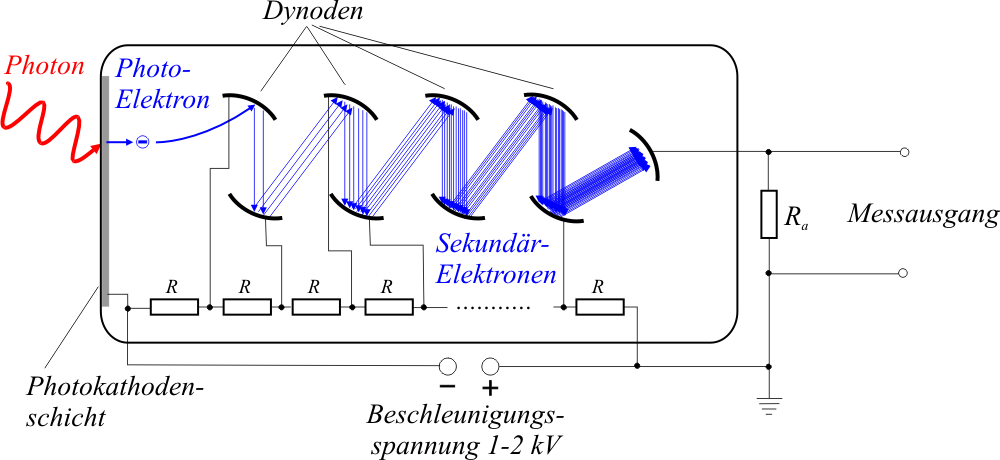
\includegraphics[scale=1]{pics/Photomultiplier_schema_de.png}
\caption{Schematischer Aufbau eines PMT. Quelle: \cite{Jkrieger.}}
\end{figure}
Die Grenzbereiche der spektrale Empfindlichkeit von Photokathoden liegen im ultravioletten und im infraroten Bereich. Ein Photokathodenmaterial zeichnet sich durch eine hohe Quanteneffizienz aus. Diese gibt die Wahrscheinlichkeit an, mit der ein auftreffendes Photon ein Photoelektron loslöst. Als Kathodenmaterial wird meistens Cäsium eingesetzt, da es von allen Elementen mit 1,9eV die geringste Austrittsarbeit hat. Durch eine geringere Austrittsarbeit wird eine Photokathode für größere Wellenlängen und somit für sichtbares Licht empfindlich. Cäsium bietet zudem eine Quanteneffizienz von ca. 30$\%$ was vergleichsweise ein sehr hoher Wert ist.

\subsection{Constant Fraction Discriminator (CFD)}
Vom Photoelektronenvervielfacher gehen die Impulse in den CFD dieser gibt einen kurzen (Dauer ca. 10-20ns) Puls als Zeichen der Detektion und ein längeren Puls (mehrere ms lang) zur Feststellung der Energie der Auslösung. Der Unterschied zu anderen Diskriminatoren besteht in der Art der Auslösung. Ein herkömmlicher Diskriminator löst bei einem besteimmten Schwellwert aus. Das hat den Nachteil, das zwei Pulse mit selber Anstiegszeit aber unterschiedlicher Amplitude zu unterschiedlichen Zeitpunkten registriert und somit weitergeleitet werden. Der CFD löst hingegen dann aus, wenn ein fester Bruchteil, hier 40\% der Anstiegszeit vergangen ist. Das funktioniert über ein im Abb.(\ref{img:CFD}) gezeigtes Prinzip.
\bild{0.7}{CFD}{in a) ist die Funktionsweise des CFD dargestellt. b) ist ein Vergleich von herkömmlichem Diskriminator links, und CFD rechts}
\subsection{Koinzidenz}
Beim Versuch werden je zwei Szintillatoren und Photoelektronenverfielfacher zur Detektion an zwei Orten zur selben zeit gebraucht. Um herauszufinden, wann beide Detektoren gleichzeitig ausgelöst haben, braucht man eine Koinzidenzschaltung. Wir sind ausschließlich an den kurzen Pulsen aus dem CFD interessiert. Da diese eine Dauer von nur etwa 10-20ns haben wirken sich die Länge oder minimale Unterschiede in der Verschaltung der beiden CFD's bereits stark auf die Ankunft des Signals in der Koinzidenzschaltung (eigentlich Slow-Fast-Koinzidenz, da auch die langsamen Signale vom CFD erkannt werden, hier aber unerheblich) aus. Um den Vorsprung den der eine Puls durch ein womöglich kürzeres Kabel gegenüber dem anderen eigentlich aber zeitgleichem Impuls am Messpunkt der Koinzidenz hat, lässt sich dieser verzögern um bis zu einige 100 ns. Zudem lässt sich die Zeitspanne variieren in der die Koinzidenz zwei Pulse als gleichzeitig wertet. Problematisch ist, dass auch durch Zufall zwei eigentlich unabhängige Impulse gleichzeitig auslösen und somit von der Koinzidenz als Messwerte gezählt werden. In der Auswertung des Versuches werden wir einen Weg finden dieses Problem zu lösen.

\subsection{aisuda}
asodaidjm oasdm iosnc i u in di  dn idndnasi cin cuin uin sdnoish dionds  sid sdisd j sduiaisaisadjkasias dis diasdasd askdi iasd saiodn i d dasd ajsiduasidnaisd asd 
\newpage
\nocite{Schatz.2008}
\nocite{Wikipedia.2014}
\printbibliography

\newpage
\begin{appendix}
\section{}

\end{appendix}
\end{document} 
